% Options for packages loaded elsewhere
\PassOptionsToPackage{unicode}{hyperref}
\PassOptionsToPackage{hyphens}{url}
%
\documentclass[
]{book}
\usepackage{amsmath,amssymb}
\usepackage{lmodern}
\usepackage{ifxetex,ifluatex}
\ifnum 0\ifxetex 1\fi\ifluatex 1\fi=0 % if pdftex
  \usepackage[T1]{fontenc}
  \usepackage[utf8]{inputenc}
  \usepackage{textcomp} % provide euro and other symbols
\else % if luatex or xetex
  \usepackage{unicode-math}
  \defaultfontfeatures{Scale=MatchLowercase}
  \defaultfontfeatures[\rmfamily]{Ligatures=TeX,Scale=1}
\fi
% Use upquote if available, for straight quotes in verbatim environments
\IfFileExists{upquote.sty}{\usepackage{upquote}}{}
\IfFileExists{microtype.sty}{% use microtype if available
  \usepackage[]{microtype}
  \UseMicrotypeSet[protrusion]{basicmath} % disable protrusion for tt fonts
}{}
\makeatletter
\@ifundefined{KOMAClassName}{% if non-KOMA class
  \IfFileExists{parskip.sty}{%
    \usepackage{parskip}
  }{% else
    \setlength{\parindent}{0pt}
    \setlength{\parskip}{6pt plus 2pt minus 1pt}}
}{% if KOMA class
  \KOMAoptions{parskip=half}}
\makeatother
\usepackage{xcolor}
\IfFileExists{xurl.sty}{\usepackage{xurl}}{} % add URL line breaks if available
\IfFileExists{bookmark.sty}{\usepackage{bookmark}}{\usepackage{hyperref}}
\hypersetup{
  pdftitle={UNDER CONSTRUCTION},
  pdfauthor={Philip Leftwich},
  hidelinks,
  pdfcreator={LaTeX via pandoc}}
\urlstyle{same} % disable monospaced font for URLs
\usepackage{color}
\usepackage{fancyvrb}
\newcommand{\VerbBar}{|}
\newcommand{\VERB}{\Verb[commandchars=\\\{\}]}
\DefineVerbatimEnvironment{Highlighting}{Verbatim}{commandchars=\\\{\}}
% Add ',fontsize=\small' for more characters per line
\usepackage{framed}
\definecolor{shadecolor}{RGB}{248,248,248}
\newenvironment{Shaded}{\begin{snugshade}}{\end{snugshade}}
\newcommand{\AlertTok}[1]{\textcolor[rgb]{0.94,0.16,0.16}{#1}}
\newcommand{\AnnotationTok}[1]{\textcolor[rgb]{0.56,0.35,0.01}{\textbf{\textit{#1}}}}
\newcommand{\AttributeTok}[1]{\textcolor[rgb]{0.77,0.63,0.00}{#1}}
\newcommand{\BaseNTok}[1]{\textcolor[rgb]{0.00,0.00,0.81}{#1}}
\newcommand{\BuiltInTok}[1]{#1}
\newcommand{\CharTok}[1]{\textcolor[rgb]{0.31,0.60,0.02}{#1}}
\newcommand{\CommentTok}[1]{\textcolor[rgb]{0.56,0.35,0.01}{\textit{#1}}}
\newcommand{\CommentVarTok}[1]{\textcolor[rgb]{0.56,0.35,0.01}{\textbf{\textit{#1}}}}
\newcommand{\ConstantTok}[1]{\textcolor[rgb]{0.00,0.00,0.00}{#1}}
\newcommand{\ControlFlowTok}[1]{\textcolor[rgb]{0.13,0.29,0.53}{\textbf{#1}}}
\newcommand{\DataTypeTok}[1]{\textcolor[rgb]{0.13,0.29,0.53}{#1}}
\newcommand{\DecValTok}[1]{\textcolor[rgb]{0.00,0.00,0.81}{#1}}
\newcommand{\DocumentationTok}[1]{\textcolor[rgb]{0.56,0.35,0.01}{\textbf{\textit{#1}}}}
\newcommand{\ErrorTok}[1]{\textcolor[rgb]{0.64,0.00,0.00}{\textbf{#1}}}
\newcommand{\ExtensionTok}[1]{#1}
\newcommand{\FloatTok}[1]{\textcolor[rgb]{0.00,0.00,0.81}{#1}}
\newcommand{\FunctionTok}[1]{\textcolor[rgb]{0.00,0.00,0.00}{#1}}
\newcommand{\ImportTok}[1]{#1}
\newcommand{\InformationTok}[1]{\textcolor[rgb]{0.56,0.35,0.01}{\textbf{\textit{#1}}}}
\newcommand{\KeywordTok}[1]{\textcolor[rgb]{0.13,0.29,0.53}{\textbf{#1}}}
\newcommand{\NormalTok}[1]{#1}
\newcommand{\OperatorTok}[1]{\textcolor[rgb]{0.81,0.36,0.00}{\textbf{#1}}}
\newcommand{\OtherTok}[1]{\textcolor[rgb]{0.56,0.35,0.01}{#1}}
\newcommand{\PreprocessorTok}[1]{\textcolor[rgb]{0.56,0.35,0.01}{\textit{#1}}}
\newcommand{\RegionMarkerTok}[1]{#1}
\newcommand{\SpecialCharTok}[1]{\textcolor[rgb]{0.00,0.00,0.00}{#1}}
\newcommand{\SpecialStringTok}[1]{\textcolor[rgb]{0.31,0.60,0.02}{#1}}
\newcommand{\StringTok}[1]{\textcolor[rgb]{0.31,0.60,0.02}{#1}}
\newcommand{\VariableTok}[1]{\textcolor[rgb]{0.00,0.00,0.00}{#1}}
\newcommand{\VerbatimStringTok}[1]{\textcolor[rgb]{0.31,0.60,0.02}{#1}}
\newcommand{\WarningTok}[1]{\textcolor[rgb]{0.56,0.35,0.01}{\textbf{\textit{#1}}}}
\usepackage{longtable,booktabs,array}
\usepackage{calc} % for calculating minipage widths
% Correct order of tables after \paragraph or \subparagraph
\usepackage{etoolbox}
\makeatletter
\patchcmd\longtable{\par}{\if@noskipsec\mbox{}\fi\par}{}{}
\makeatother
% Allow footnotes in longtable head/foot
\IfFileExists{footnotehyper.sty}{\usepackage{footnotehyper}}{\usepackage{footnote}}
\makesavenoteenv{longtable}
\usepackage{graphicx}
\makeatletter
\def\maxwidth{\ifdim\Gin@nat@width>\linewidth\linewidth\else\Gin@nat@width\fi}
\def\maxheight{\ifdim\Gin@nat@height>\textheight\textheight\else\Gin@nat@height\fi}
\makeatother
% Scale images if necessary, so that they will not overflow the page
% margins by default, and it is still possible to overwrite the defaults
% using explicit options in \includegraphics[width, height, ...]{}
\setkeys{Gin}{width=\maxwidth,height=\maxheight,keepaspectratio}
% Set default figure placement to htbp
\makeatletter
\def\fps@figure{htbp}
\makeatother
\setlength{\emergencystretch}{3em} % prevent overfull lines
\providecommand{\tightlist}{%
  \setlength{\itemsep}{0pt}\setlength{\parskip}{0pt}}
\setcounter{secnumdepth}{5}
\usepackage{booktabs}
\usepackage{amsthm}
\makeatletter
\def\thm@space@setup{%
  \thm@preskip=8pt plus 2pt minus 4pt
  \thm@postskip=\thm@preskip
}
\makeatother
\usepackage{booktabs}
\usepackage{longtable}
\usepackage{array}
\usepackage{multirow}
\usepackage{wrapfig}
\usepackage{float}
\usepackage{colortbl}
\usepackage{pdflscape}
\usepackage{tabu}
\usepackage{threeparttable}
\usepackage{threeparttablex}
\usepackage[normalem]{ulem}
\usepackage{makecell}
\usepackage{xcolor}
\ifluatex
  \usepackage{selnolig}  % disable illegal ligatures
\fi
\usepackage[]{natbib}
\bibliographystyle{apalike}

\title{UNDER CONSTRUCTION}
\author{Philip Leftwich}
\date{2021-04-20}

\begin{document}
\maketitle

{
\setcounter{tocdepth}{1}
\tableofcontents
}
\hypertarget{introduction}{%
\chapter{Introduction}\label{introduction}}

This is a \emph{sample} book written in \textbf{Markdown}. You can use anything that Pandoc's Markdown supports, e.g., a math equation \(a^2 + b^2 = c^2\).

The \textbf{bookdown} package can be installed from CRAN or Github:

\begin{Shaded}
\begin{Highlighting}[]
\FunctionTok{install.packages}\NormalTok{(}\StringTok{"bookdown"}\NormalTok{)}
\CommentTok{\# or the development version}
\CommentTok{\# devtools::install\_github("rstudio/bookdown")}
\end{Highlighting}
\end{Shaded}

Remember each Rmd file contains one and only one chapter, and a chapter is defined by the first-level heading \texttt{\#}.

To compile this example to PDF, you need XeLaTeX. You are recommended to install TinyTeX (which includes XeLaTeX): \url{https://yihui.name/tinytex/}.

\hypertarget{Unix}{%
\chapter{Unix}\label{Unix}}

Unix is very likely the most foundational skillset we can develop for bioinformatics (and much more than bioinformatics). Many of the most common and powerful bioinformatics approaches happen in this text-based environment, and having a solid foundation here can make everything we're trying to learn and do much easier. This is a set of 5 introductory tutorials to help us get from being completely new to Unix up to being great friends with it 🙂

\hypertarget{what-is-unixlinux}{%
\section{What is Unix/Linux}\label{what-is-unixlinux}}

\hypertarget{some-terms}{%
\subsection{Some terms}\label{some-terms}}

Here are some terms worth knowing, don't worry about memorising them, it can just be useful to have these to refer to in the future.

\begin{longtable}{ll}
\toprule
\textbf{Term} & \textbf{What it is}\\
\midrule
shell & what we use to talk to the computer; anything where you are pointing and clicking with a mouse is a Graphical User Interface (GUI) shell; something with text only is a Command Line Interface (CLI) shell\\
command line & a text-based environment capable of taking input and providing output\\
Unix & a family of operating systems (we also use the term “Unix-like” because one of the most popular operating systems derived from Unix is specifically named as not being Unix)\\
bash & the most common programming language used at a Unix command-line\\
\bottomrule
\end{longtable}

You should be very familiar with using a GUI (RStudio), but remember we have spent a lot of time working with files and directories using the the command line (CLI) in R. This is useful practice, because most supercomputers lack a GUI, you must work entirely using the command line.

\hypertarget{why-learn-unix}{%
\section{Why Learn Unix?}\label{why-learn-unix}}

Most sequencing data files are large, and require a lot of RAM to process. As a result most of the work Bioinformaticians do is not hosted on their own computers, instead they ``remote-connect'' to high performance supercomputers or cluster computers.

The Linux Operating System is highly flexible, free, open-source (like R) and uses very little RAM to run (Unlike Windows OS) - as such you find most supercomputers run on Linux.

You already have some experience with using a Linux OS - every time you log into RStudio Cloud you are connecting to a supercomputer that runs on Linux. Normally we do not interact directly with the OS, instead we use R and RStudio directly.

But when you click on the RStudio Terminal it provides direct access to a command-line where we can execute commands and functions directly in Linux.

This allows us to start using programs other than R, and potentially use multiple programs \& programming languages to work together.

\hypertarget{note-this-series-of-practicals-is-designed-for-you-to-have-a-first-introduction-to-bioinformatics-its-about-exposure-not-memorising-or-mastering-anything.-dont-worry-about-the-details}{%
\subsection{Note this series of practicals is designed for you to have a first introduction to Bioinformatics, it's about exposure, not memorising or mastering anything. Don't worry about the details!}\label{note-this-series-of-practicals-is-designed-for-you-to-have-a-first-introduction-to-bioinformatics-its-about-exposure-not-memorising-or-mastering-anything.-dont-worry-about-the-details}}

\hypertarget{getting-started}{%
\section{Getting started}\label{getting-started}}

Before we get started we need a terminal to work in.

\begin{itemize}
\item
  Open the Bioinformatics RStudio Cloud Project in the 5023Y workspace
\item
  Click on the Terminal tab next to console in the bottom-left pane of the RStudio GUI
\end{itemize}

\begin{Shaded}
\begin{Highlighting}[]
\FunctionTok{par}\NormalTok{(}\AttributeTok{mar =} \FunctionTok{c}\NormalTok{(}\DecValTok{4}\NormalTok{, }\DecValTok{4}\NormalTok{, .}\DecValTok{1}\NormalTok{, .}\DecValTok{1}\NormalTok{))}
\FunctionTok{plot}\NormalTok{(pressure, }\AttributeTok{type =} \StringTok{\textquotesingle{}b\textquotesingle{}}\NormalTok{, }\AttributeTok{pch =} \DecValTok{19}\NormalTok{)}
\end{Highlighting}
\end{Shaded}

\begin{figure}

{\centering 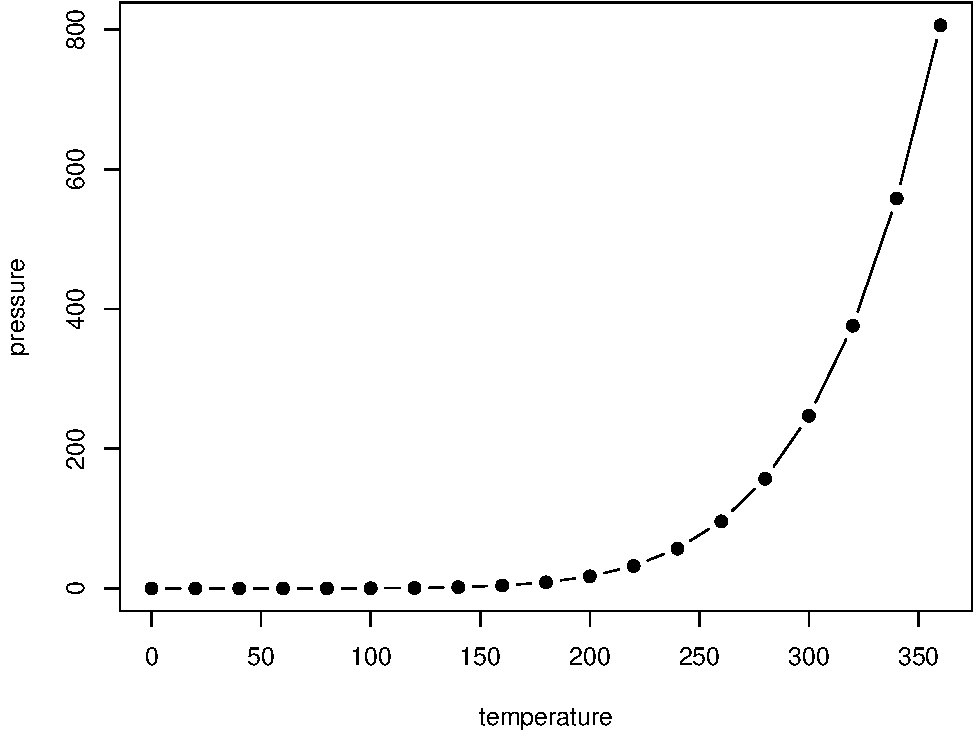
\includegraphics[width=0.8\linewidth]{bookdown-demo_files/figure-latex/nice-fig-1} 

}

\caption{Here is a nice figure!}\label{fig:nice-fig}
\end{figure}

\begin{itemize}
\item
  This is our ``command line'' where we will be typing all of our commands.
\item
  If you need to, you can exit the Terminal and start a new session easily with options in RStudio
\end{itemize}

\hypertarget{a-few-foundational-rules}{%
\section{1.4 A few foundational rules}\label{a-few-foundational-rules}}

\begin{itemize}
\item
  Just like in R spaces are special, spaces break things apart, as a rule it is therefore better to have functions and file names with dashes (-) or underscores (\_) - e.g.~``draft\_v3.txt'' is preferred to ``draft v3.txt''.
\item
  The general syntax on the command line is: \texttt{command} \texttt{argument}. Again this is very similar to R except we don't use brackets e.g.~R we are used to \texttt{command(argument)}
\item
  Arguments can be \textbf{optional} e.g.~if their is a default argument you may not have to write anything. Some functions \emph{require} that arguments are specified. Again this is just like R.
\end{itemize}

\hypertarget{lets-get-started}{%
\section{1.5 Let's get started}\label{lets-get-started}}

We will perform a very simple function and get a flavour of the similarities and differences to working in `\texttt{R}. date` is a command that prints out the date and time.

\begin{Shaded}
\begin{Highlighting}[]
    \FunctionTok{date}
\end{Highlighting}
\end{Shaded}

\url{https://www.geeksforgeeks.org/date-command-linux-examples/\#}:\textasciitilde:text=date\%20command\%20is\%20used\%20to,linux\%20operating\%20system\%20is\%20configured.

\begin{Shaded}
\begin{Highlighting}[]
    \VariableTok{TZ=}\NormalTok{Europe/London }\FunctionTok{date}

    \VariableTok{TZ=}\NormalTok{Europe/London }\FunctionTok{date}

    \FunctionTok{date} \AttributeTok{{-}{-}date}\OperatorTok{=}\StringTok{"next tue"}
\end{Highlighting}
\end{Shaded}

\hypertarget{downloading-data}{%
\subsection{Downloading data}\label{downloading-data}}

\begin{itemize}
\item
  curl is a command line tool for transferring data to and from the server here we will use this to download data from an online repository.
\item
  tar will \emph{unpack} the data from a compressed file format
\item
  cd change the directory so we \emph{land} in the new folder we have made
\end{itemize}

\begin{Shaded}
\begin{Highlighting}[]
    \ExtensionTok{curl} \AttributeTok{{-}L} \AttributeTok{{-}o}\NormalTok{ unix\_intro.tar.gz https://ndownloader.figshare.com/files/15573746}
    \FunctionTok{tar} \AttributeTok{{-}xzvf}\NormalTok{ unix\_intro.tar.gz }\KeywordTok{\&\&} \FunctionTok{rm}\NormalTok{ unix\_intro.tar.gz}
    \BuiltInTok{cd}\NormalTok{ unix\_intro}
\end{Highlighting}
\end{Shaded}

Unlike date, most commands require arguments and won't work without them. head is a command that prints the first lines of a file, so it requires us to provide the file we want it to act on:

\begin{Shaded}
\begin{Highlighting}[]
    \FunctionTok{head}\NormalTok{ example.txt}
\end{Highlighting}
\end{Shaded}

Here ``example.txt'' is the required argument, and in this case it is also what's known as a positional argument. Whether things need to be provided as positional arguments or not depends on how the command or program we are using was written. Sometimes we need to specify the input file by putting something in front of it (e.g.~some commands will use the -i flag, but it's often other things as well).

There are also optional arguments for the head command. The default for head is to print the first 10 lines of a file. We can change that by specifying the -n flag, followed by how many lines we want:

\begin{Shaded}
\begin{Highlighting}[]
    \FunctionTok{head} \AttributeTok{{-}n}\NormalTok{ 5 example.txt}
\end{Highlighting}
\end{Shaded}

How would we know we needed the -n flag for that? There are a few ways to find out. Many standard Unix commands and other programs will have built-in help menus that we can access by providing --help as the only argument:

\begin{Shaded}
\begin{Highlighting}[]
    \FunctionTok{head} \AttributeTok{{-}{-}help}
\end{Highlighting}
\end{Shaded}

Again this is very similar to the logic in which R commands are strucutred e.g.~\texttt{??ggplot()} The synatx is similar even if the specific icons or arguments are different.

Remember just like with R, one of your best friends is Google! As you get familiar with any language or OS we might remember a few flags or specific options, but searching for options and details when needed is definitely the norm!

\hypertarget{unix-file-structure}{%
\section{1.6 Unix File Structure}\label{unix-file-structure}}

There are two special locations in all Unix-based systems: the ``root'' location and the current user's ``home'' location. ``Root'' is where the address system of the computer starts; ``home'' is where the current user's location starts.

IMAGE

We tell the command line where files and directories are located by providing their address, their ``path''. If we use the pwd command (for print working directory), we can find out what the path is for the directory we are sitting in. And if we use the ls command (for list), we can see what directories and files are in the current directory we are sitting in.

\begin{Shaded}
\begin{Highlighting}[]
    \BuiltInTok{pwd}
    \FunctionTok{ls}
\end{Highlighting}
\end{Shaded}

\hypertarget{absolute-vs-relative-file-paths}{%
\section{1.7 Absolute vs relative file paths}\label{absolute-vs-relative-file-paths}}

You should be used to these concepts from your work with R projects.

There are two ways to specify the path (address) of the file we want to do something to:

\begin{itemize}
\item
  An \textbf{absolute path} is an address that starts from an explicitly specified location: either the ``root'' \texttt{/} or the ``home'' \texttt{\textasciitilde{}/} location. (Side note, because we also may see or hear the term, the ``full path'', is the absolute path that starts from the ``root'' /.)
\item
  A \textbf{relative path} is an address that starts from wherever we are currently sitting. For example, let's look again at the head command we ran above:
\end{itemize}

\begin{Shaded}
\begin{Highlighting}[]
    \FunctionTok{head}\NormalTok{ example.txt}
\end{Highlighting}
\end{Shaded}

What we are actually doing here is using a relative path to specify where the ``example.txt'' file is located. This is because the command line \textbf{automatically looks} in the current working directory if we don't specify anything else about its location.

We can also run the same command on the same file using an \textbf{absolute path}:

\begin{Shaded}
\begin{Highlighting}[]
    \FunctionTok{head}\NormalTok{ \textasciitilde{}/unix\_intro/example.txt}
\end{Highlighting}
\end{Shaded}

The previous two commands both point to the same file right now. But the first way, head example.txt, will only work if we are entering it while ``sitting'' in the directory that holds that file, while the second way will work no matter where we happen to be in the computer.

It is \textbf{important to always think about where} we are in the computer when working at the command line. One of the most common errors/easiest mistakes to make is trying to do something to a file that isn't where we think it is. Let's run head on the ``example.txt'' file again, and then let's try it on another file: ``notes.txt'':

\begin{Shaded}
\begin{Highlighting}[]
\FunctionTok{head}\NormalTok{ example.txt}
\FunctionTok{head}\NormalTok{ notes.txt}
\end{Highlighting}
\end{Shaded}

Here the head command works fine on ``example.txt'', but we get an error message when we call it on ``notes.txt'' telling us no such file or directory. If we run the ls command to list the contents of the current working directory, we can see the computer is absolutely right -- spoiler alert: it usually is -- and there is no file here named ``notes.txt''.

The ls command by default operates on the current working directory if we don't specify any location, but we can tell it to list the contents of a different directory by providing it as a positional argument:

\begin{Shaded}
\begin{Highlighting}[]
    \FunctionTok{ls}
    \FunctionTok{ls}\NormalTok{ experiment}
\end{Highlighting}
\end{Shaded}

We can see the file we were looking for is located in the subdirectory called ``experiment''. Here is how we can run head on ``notes.txt'' by specifying an accurate relative path to that file:

\begin{Shaded}
\begin{Highlighting}[]
    \FunctionTok{head}\NormalTok{ experiment/notes.txt}
\end{Highlighting}
\end{Shaded}

\hypertarget{moving-around}{%
\section{1.8 Moving around}\label{moving-around}}

We can also move into the directory containing the file we want to work with by using the \texttt{cd} command (\textbf{c}hange \textbf{d}irectory). This command takes a positional argument that is the path (address) of the directory we want to change into. This can be a relative path or an absolute path. Here we'll use the relative path of the subdirectory, ``experiment'', to change into it

\begin{Shaded}
\begin{Highlighting}[]
    \BuiltInTok{cd}\NormalTok{ experiment/}
    \BuiltInTok{pwd}
    \FunctionTok{ls}
    \FunctionTok{head}\NormalTok{ notes.txt}
\end{Highlighting}
\end{Shaded}

Great. But now how do we get back ``up'' to the directory above us? One way would be to provide an absolute path, like \texttt{cd\ \textasciitilde{}/unix\_intro}, but there is also a handy shortcut. \texttt{..} are special characters that act as a relative path specifying ``up'' one level -- one directory -- from wherever we currently are. So we can provide that as the positional argument to cd to get back to where we started:

\begin{Shaded}
\begin{Highlighting}[]
    \BuiltInTok{cd}\NormalTok{ ..}
    \BuiltInTok{pwd}
    \FunctionTok{ls}
\end{Highlighting}
\end{Shaded}

Moving around the computer like this might feel a bit cumbersome and frustrating at first, but after spending a little time with it, you will get used to it, and it starts to feel more natural.

Get used to using \textbf{tab} to perform \textbf{tab-completion} often this will auto-complete file names!

\begin{itemize}
\tightlist
\item
  Press tab twice quickly and it will print all possible combinations
\end{itemize}

\hypertarget{summary}{%
\section{1.9 Summary}\label{summary}}

While maybe not all that exciting, these things really are the foundation needed to start utilizing the command line -- which then gives us the capability to use lots of tools that only work at a command line, manipulate large files rapidly, access and work with remote computers, and more! These are the fundamental tools that every scientist needs to work with \textbf{big data}.

\hypertarget{terms}{%
\subsection{Terms}\label{terms}}

\begin{longtable}{ll}
\toprule
\textbf{Term} & \textbf{What it is}\\
\midrule
path & the address system the computer uses to keep track of files and directories\\
root & where the address system of the computer starts, /\\
home & where the current user’s location starts, \textasciitilde{}/\\
absolute path & an address that starts from a specified location, i.e. root, or home\\
relative path & an address that starts from wherever we are\\
\addlinespace
tab-completion & our best friend\\
\bottomrule
\end{longtable}

\hypertarget{commands}{%
\subsection{Commands}\label{commands}}

\begin{longtable}{ll}
\toprule
\textbf{Command} & \textbf{What it is}\\
\midrule
date & prints out information about the current date and time\\
head & prints out the first lines of a file\\
pwd & prints out where we are in the computer (print working directory)\\
ls & lists contents of a directory (list)\\
cd & change directories\\
\bottomrule
\end{longtable}

\hypertarget{special-characters}{%
\subsection{Special characters}\label{special-characters}}

\begin{longtable}{ll}
\toprule
\textbf{Command} & \textbf{What it is}\\
\midrule
Characters & Meaning\\
/ & the computer’s root location\\
\textasciitilde{}/ & the user’s home location\\
../ & specifies a directory one level “above” the current working directory\\
\bottomrule
\end{longtable}

\hypertarget{stretch-yourself}{%
\section{1.10 Stretch yourself}\label{stretch-yourself}}

\url{https://bioinformaticsworkbook.org/Appendix/Unix/unix-basics-1.html\#gsc.tab=0}

\url{http://evomics.org/learning/unix-tutorial/}

Reference a figure by its code chunk label with the \texttt{fig:} prefix, e.g., see Figure \ref{fig:nice-fig}. Similarly, you can reference tables generated from \texttt{knitr::kable()}, e.g., see Table \ref{tab:nice-tab}.

\begin{Shaded}
\begin{Highlighting}[]
\NormalTok{knitr}\SpecialCharTok{::}\FunctionTok{kable}\NormalTok{(}
  \FunctionTok{head}\NormalTok{(iris, }\DecValTok{20}\NormalTok{), }\AttributeTok{caption =} \StringTok{\textquotesingle{}Here is a nice table!\textquotesingle{}}\NormalTok{,}
  \AttributeTok{booktabs =} \ConstantTok{TRUE}
\NormalTok{)}
\end{Highlighting}
\end{Shaded}

\begin{table}

\caption{\label{tab:nice-tab}Here is a nice table!}
\centering
\begin{tabular}[t]{rrrrl}
\toprule
Sepal.Length & Sepal.Width & Petal.Length & Petal.Width & Species\\
\midrule
5.1 & 3.5 & 1.4 & 0.2 & setosa\\
4.9 & 3.0 & 1.4 & 0.2 & setosa\\
4.7 & 3.2 & 1.3 & 0.2 & setosa\\
4.6 & 3.1 & 1.5 & 0.2 & setosa\\
5.0 & 3.6 & 1.4 & 0.2 & setosa\\
\addlinespace
5.4 & 3.9 & 1.7 & 0.4 & setosa\\
4.6 & 3.4 & 1.4 & 0.3 & setosa\\
5.0 & 3.4 & 1.5 & 0.2 & setosa\\
4.4 & 2.9 & 1.4 & 0.2 & setosa\\
4.9 & 3.1 & 1.5 & 0.1 & setosa\\
\addlinespace
5.4 & 3.7 & 1.5 & 0.2 & setosa\\
4.8 & 3.4 & 1.6 & 0.2 & setosa\\
4.8 & 3.0 & 1.4 & 0.1 & setosa\\
4.3 & 3.0 & 1.1 & 0.1 & setosa\\
5.8 & 4.0 & 1.2 & 0.2 & setosa\\
\addlinespace
5.7 & 4.4 & 1.5 & 0.4 & setosa\\
5.4 & 3.9 & 1.3 & 0.4 & setosa\\
5.1 & 3.5 & 1.4 & 0.3 & setosa\\
5.7 & 3.8 & 1.7 & 0.3 & setosa\\
5.1 & 3.8 & 1.5 & 0.3 & setosa\\
\bottomrule
\end{tabular}
\end{table}

You can write citations, too. For example, we are using the \textbf{bookdown} package \citep{R-bookdown} in this sample book, which was built on top of R Markdown and \textbf{knitr} \citep{xie2015}.

\hypertarget{ngs-sequence-analysis}{%
\chapter{NGS sequence analysis}\label{ngs-sequence-analysis}}

\hypertarget{background}{%
\section{Background}\label{background}}

Info on sequencing

General application

Don't have to follow everything!

\hypertarget{the-data}{%
\section{The data}\label{the-data}}

For a quick overview of the example data we'll be using and where it came from, we are going to work with a subset of the dataset published here. We were exploring an underwater mountain \textasciitilde3 km down at the bottom of the Pacific Ocean that serves as a low-temperature (\textasciitilde5-10°C) hydrothermal venting site. This amplicon dataset was generated from DNA extracted from crushed basalts collected from across the mountain with the goal being to begin characterizing the microbial communities of these deep-sea rocks. No one had ever been here before, so as is often the purpose of marker-gene sequencing, this was just a broad-level community survey. The sequencing was done on the Illumina MiSeq platform with 2x300 paired-end sequencing using primers targeting the V4 region of the 16S rRNA gene. There are 20 samples total: 4 extraction ``blanks'' (nothing added to DNA extraction kit), 2 bottom-water samples, 13 rocks, and one biofilm scraped off of a rock. None of these details are important for you to remember, it's just to give some overview if you care.

In the following figure, overlain on the map are the rock sample collection locations, and the panes on the right show examples of the 3 distinct types of rocks collected: 1) basalts with highly altered, thick outer rinds (\textgreater1 cm); 2) basalts that were smooth, glassy, thin exteriors (\textasciitilde1-2 mm); and 3) one calcified carbonate.

PICTURE

Altogether the uncompressed size of the working directory we are downloading here is \textasciitilde300MB - this is about 10\% of the full dataset - we are using a reduced dataset to minimise system requirements and speed up the workflow.

To get started, be sure you are in the ``Terminal'' window. We will be working here for the first step of importing the data, and removing the primers from our data. We can import our data using the \texttt{curl} function, we will then remove the primers using a program called \texttt{cutadapt} which is written in Python.

Make sure when you open the terminal you are in the project directory (and refer to last weeks notes if you need to check how to do this).

Don't switch over to R (the ``Console'' tab in the Binder/RStudio environment) until noted. You can download the required dataset and files by copying and pasting the following commands into your command-line terminal:

\begin{Shaded}
\begin{Highlighting}[]
    \ExtensionTok{curl} \AttributeTok{{-}L} \AttributeTok{{-}o}\NormalTok{ dada2\_amplicon\_ex\_workflow.tar.gz https://ndownloader.figshare.com/files/23066516}
    \FunctionTok{tar} \AttributeTok{{-}xzvf}\NormalTok{ dada2\_amplicon\_ex\_workflow.tar.gz}
    \FunctionTok{rm}\NormalTok{ dada2\_amplicon\_ex\_workflow.tar.gz}
    \BuiltInTok{cd}\NormalTok{ dada2\_amplicon\_ex\_workflow/}
\end{Highlighting}
\end{Shaded}

In our working directory there are 20 samples with forward (R1) and reverse (R2) reads with per-base-call quality information, so 40 fastq files (.fq). It is a good idea to have a file with all the sample names to use for various things throughout, so here's making that file based on how these sample names are formatted.

\begin{Shaded}
\begin{Highlighting}[]
    \FunctionTok{ls} \PreprocessorTok{*}\NormalTok{\_R1.fq }\KeywordTok{|} \FunctionTok{cut} \AttributeTok{{-}f1} \AttributeTok{{-}d} \StringTok{"\_"} \OperatorTok{\textgreater{}}\NormalTok{ samples}
\end{Highlighting}
\end{Shaded}

\hypertarget{removing-primers}{%
\section{Removing Primers}\label{removing-primers}}

To start, we need to remove the primers from all of these (the primers used for this run are in the ``primers.fa'' file in our working directory), and here we're going to use cutadapt to do that at the command line (``Terminal'' tab). Cutadapt operates on one sample at at time, so we're going to use a wonderful little bash \emph{loop} to run it on all of our samples.

\hypertarget{loops}{%
\subsection{Loops}\label{loops}}

Loops are extremely powerful way of controlling iteration. We can specify that a line of code is repeated across multiple objects. In this example we use the sample file we made earlier as the list of files across which we want this function of removing primers to loop. These same lines will then repeat until all the specified iterations are complete.

We won't break down exactly how this loop works - but they are used across all programming languages (including R) and you can check out the R4DS book for an introduction to building your own loops (and custom functions!) \href{https://r4ds.had.co.nz/iteration.html}{here}.

For now just copy and paste this code exactly into the Terminal.

\begin{Shaded}
\begin{Highlighting}[]
    \ControlFlowTok{for}\NormalTok{ sample }\KeywordTok{in} \VariableTok{$(}\FunctionTok{cat}\NormalTok{ samples}\VariableTok{)}
    \ControlFlowTok{do}

        \BuiltInTok{echo} \StringTok{"On sample: }\VariableTok{$sample}\StringTok{"}
        
        \ExtensionTok{cutadapt} \AttributeTok{{-}a}\NormalTok{ \^{}GTGCCAGCMGCCGCGGTAA...ATTAGAWACCCBDGTAGTCC }\DataTypeTok{\textbackslash{}}
        \AttributeTok{{-}A}\NormalTok{ \^{}GGACTACHVGGGTWTCTAAT...TTACCGCGGCKGCTGGCAC }\DataTypeTok{\textbackslash{}}
        \AttributeTok{{-}m}\NormalTok{ 215 }\AttributeTok{{-}M}\NormalTok{ 285 }\AttributeTok{{-}{-}discard{-}untrimmed} \DataTypeTok{\textbackslash{}}
        \AttributeTok{{-}o} \VariableTok{$\{sample\}}\NormalTok{\_sub\_R1\_trimmed.fq.gz }\AttributeTok{{-}p} \VariableTok{$\{sample\}}\NormalTok{\_sub\_R2\_trimmed.fq.gz }\DataTypeTok{\textbackslash{}}
        \VariableTok{$\{sample\}}\NormalTok{\_sub\_R1.fq }\VariableTok{$\{sample\}}\NormalTok{\_sub\_R2.fq }\DataTypeTok{\textbackslash{}}
        \OperatorTok{\textgreater{}\textgreater{}}\NormalTok{ cutadapt\_primer\_trimming\_stats.txt }\DecValTok{2}\OperatorTok{\textgreater{}\&}\DecValTok{1}

    \ControlFlowTok{done}
\end{Highlighting}
\end{Shaded}

Here's a before-and-after of one of our files

\begin{verbatim}
### R1 BEFORE TRIMMING PRIMERS
head -n 2 B1_sub_R1.fq
# @M02542:42:000000000-ABVHU:1:1101:8823:2303 1:N:0:3
# GTGCCAGCAGCCGCGGTAATACGTAGGGTGCGAGCGTTAATCGGAATTACTGGGCGTAAAGCGTGCGCAGGCGGTCTTGT
# AAGACAGAGGTGAAATCCCTGGGCTCAACCTAGGAATGGCCTTTGTGACTGCAAGGCTGGAGTGCGGCAGAGGGGGATGG
# AATTCCGCGTGTAGCAGTGAAATGCGTAGATATGCGGAGGAACACCGATGGCGAAGGCAGTCCCCTGGGCCTGCACTGAC
# GCTCATGCACGAAAGCGTGGGGAGCAAACAGGATTAGATACCCGGGTAGTCC

### R1 AFTER TRIMMING PRIMERS
head -n 2 B1_sub_R1_trimmed.fq
# @M02542:42:000000000-ABVHU:1:1101:8823:2303 1:N:0:3
# TACGTAGGGTGCGAGCGTTAATCGGAATTACTGGGCGTAAAGCGTGCGCAGGCGGTCTTGTAAGACAGAGGTGAAATCCC
# TGGGCTCAACCTAGGAATGGCCTTTGTGACTGCAAGGCTGGAGTGCGGCAGAGGGGGATGGAATTCCGCGTGTAGCAGTG
# AAATGCGTAGATATGCGGAGGAACACCGATGGCGAAGGCAGTCCCCTGGGCCTGCACTGACGCTCATGCACGAAAGCGTG
# GGGAGCAAACAGG
\end{verbatim}

You can look through the output of the cutadapt stats file we made (``cutadapt\_primer\_trimming\_stats.txt'') to get an idea of how things went. Here's a little one-liner to look at what fraction of reads were retained in each sample (column 2) and what fraction of bps were retained in each sample (column 3):

\begin{Shaded}
\begin{Highlighting}[]
    \ExtensionTok{paste}\NormalTok{ samples }\OperatorTok{\textless{}(}\FunctionTok{grep} \StringTok{"passing"}\NormalTok{ cutadapt\_primer\_trimming\_stats.txt }\KeywordTok{|} \FunctionTok{cut} \AttributeTok{{-}f3} \AttributeTok{{-}d} \StringTok{"("} \KeywordTok{|} \FunctionTok{tr} \AttributeTok{{-}d} \StringTok{")"}\OperatorTok{)} \OperatorTok{\textless{}(}\FunctionTok{grep} \StringTok{"filtered"}\NormalTok{ cutadapt\_primer\_trimming\_stats.txt }\KeywordTok{|} \FunctionTok{cut} \AttributeTok{{-}f3} \AttributeTok{{-}d} \StringTok{"("} \KeywordTok{|} \FunctionTok{tr} \AttributeTok{{-}d} \StringTok{")"}\OperatorTok{)}
\end{Highlighting}
\end{Shaded}

\begin{verbatim}
# B1    96.5%   83.0%
# B2    96.6%   83.3%
# B3    95.4%   82.4%
# B4    96.8%   83.4%
# BW1   96.4%   83.0%
# BW2   94.6%   81.6%
# R10   92.4%   79.8%
# R11BF 90.6%   78.2%
# R11   93.3%   80.6%
# R12   94.3%   81.4%
# R1A   93.3%   80.5%
# R1B   94.0%   81.1%
# R2    94.0%   81.2%
# R3    93.8%   81.0%
# R4    95.5%   82.4%
# R5    93.7%   80.9%
# R6    92.7%   80.1%
# R7    94.4%   81.5%
# R8    93.2%   80.4%
# R9    92.4%   79.7%
\end{verbatim}

We would expect to lose around 13-14\% of bps just for cutting off the primers, and the remainder of lost bps would be from the relatively low percent of those reads totally removed (\textasciitilde92-97\% across the samples).

With primers removed, we're now ready to switch R and start using DADA2!

\hypertarget{dada2---switch-to-r-console}{%
\section{DADA2 - switch to R console}\label{dada2---switch-to-r-console}}

\begin{Shaded}
\begin{Highlighting}[]
    \FunctionTok{library}\NormalTok{(dada2)}

    \FunctionTok{setwd}\NormalTok{(}\StringTok{"\textasciitilde{}/dada2\_amplicon\_ex\_workflow"}\NormalTok{)}

    \FunctionTok{list.files}\NormalTok{() }\CommentTok{\# make sure what we think is here is actually here}

    \DocumentationTok{\#\# first we\textquotesingle{}re setting a few variables we\textquotesingle{}re going to use \#\#}
      \CommentTok{\# one with all sample names, by scanning our "samples" file we made earlier}
      
\NormalTok{    samples }\OtherTok{\textless{}{-}} \FunctionTok{scan}\NormalTok{(}\StringTok{"samples"}\NormalTok{, }\AttributeTok{what=}\StringTok{"character"}\NormalTok{)}

      \CommentTok{\# one holding the file names of all the forward reads}
\NormalTok{    forward\_reads }\OtherTok{\textless{}{-}} \FunctionTok{paste0}\NormalTok{(samples, }\StringTok{"\_sub\_R1\_trimmed.fq.gz"}\NormalTok{)}

      \CommentTok{\# and one with the reverse}
\NormalTok{    reverse\_reads }\OtherTok{\textless{}{-}} \FunctionTok{paste0}\NormalTok{(samples, }\StringTok{"\_sub\_R2\_trimmed.fq.gz"}\NormalTok{)}

      \CommentTok{\# and variables holding file names for the forward and reverse}
      \CommentTok{\# filtered reads we\textquotesingle{}re going to generate below}
\NormalTok{    filtered\_forward\_reads }\OtherTok{\textless{}{-}} \FunctionTok{paste0}\NormalTok{(samples, }\StringTok{"\_sub\_R1\_filtered.fq.gz"}\NormalTok{)}
\NormalTok{    filtered\_reverse\_reads }\OtherTok{\textless{}{-}} \FunctionTok{paste0}\NormalTok{(samples, }\StringTok{"\_sub\_R2\_filtered.fq.gz"}\NormalTok{)}
\end{Highlighting}
\end{Shaded}

\hypertarget{quality-trimmingfiltering}{%
\section{Quality trimming/filtering}\label{quality-trimmingfiltering}}

We did a filtering step above with cutadapt (where we eliminated reads that had imperfect or missing primers and those that were shorter than 215 bps or longer than 285), but in DADA2 we'll implement a trimming step as well (where we trim reads down based on some quality threshold rather than throwing the read away). Since we're potentially shortening reads further, we're again going to include another minimum-length filtering component. We can also take advantage of a handy quality plotting function that DADA2 provides to visualize how you're reads are doing, plotQualityProfile(). By running that on our variables that hold all of our forward and reverse read filenames, we can easily generate plots for all samples or for a subset of them. So let's take a peak at that to help decide our trimming lengths: It's good to try to keep a bird's-eye view of what's going on. So here is an overview of the main processing steps we'll be performing with cutadapt and DADA2. Don't worry if anything seems unclear right now, we will discuss each at each step.

\begin{Shaded}
\begin{Highlighting}[]
    \FunctionTok{plotQualityProfile}\NormalTok{(forward\_reads[}\DecValTok{17}\SpecialCharTok{:}\DecValTok{20}\NormalTok{])}

    \FunctionTok{plotQualityProfile}\NormalTok{(reverse\_reads[}\DecValTok{17}\SpecialCharTok{:}\DecValTok{20}\NormalTok{])}
\end{Highlighting}
\end{Shaded}

All forwards look pretty similar to eachother, and all reverses look pretty similar to eachother, but worse than the forwards, which is common -- chemistry gets tired\ldots{}

On the plots produced

\begin{itemize}
\item
  the x axis is the nucleotide bases starting from the beginning of the read moving to the end
\item
  the y axis is the average quality score for the base in that position
\item
  the green line is the median quality score of the base at that position
\item
  the orange lines are quartiles
\end{itemize}

TALK ABOUT PHRED SCORES

Here, I'm going to cut the forward reads at 250 and the reverse reads at 200 -- roughly where both sets maintain a median quality of 30 or above -- and then see how things look. But we also want to set a minimum length to filter out truncated sequences, so we will set a minimum acceptable read length of 175bp (any reads shorter than this will be discarded).

In DADA2, this quality-filtering step is done with the \texttt{filterAndTrim()} function:

\begin{Shaded}
\begin{Highlighting}[]
\NormalTok{    filtered\_out }\OtherTok{\textless{}{-}} \FunctionTok{filterAndTrim}\NormalTok{(forward\_reads, filtered\_forward\_reads,}
\NormalTok{                    reverse\_reads, filtered\_reverse\_reads, }\AttributeTok{maxEE=}\FunctionTok{c}\NormalTok{(}\DecValTok{2}\NormalTok{,}\DecValTok{2}\NormalTok{),}
                    \AttributeTok{rm.phix=}\ConstantTok{TRUE}\NormalTok{, }\AttributeTok{minLen=}\DecValTok{175}\NormalTok{, }\AttributeTok{truncLen=}\FunctionTok{c}\NormalTok{(}\DecValTok{250}\NormalTok{,}\DecValTok{200}\NormalTok{))}
\end{Highlighting}
\end{Shaded}

This function made a bunch of output files ``filtered\_forward\_reads'' and ``filtered\_reverse\_reads'' we can see these in our project pane. Or if we were working on a server without a GUI we could use \texttt{list.files()} in R or \texttt{ls} in our Terminal.

We also generated an R file called filtered\_out. This is a simple matrix holding how many reads went \emph{in} for each file and how many came \emph{out}.

Check it in R.

\begin{Shaded}
\begin{Highlighting}[]
\NormalTok{    filtered\_out}
\end{Highlighting}
\end{Shaded}

We can take a look at the filtered reads visually - we expect to have trimmed off that section where quality drops

\begin{Shaded}
\begin{Highlighting}[]
    \FunctionTok{plotQualityProfile}\NormalTok{(filtered\_reverse\_reads[}\DecValTok{17}\SpecialCharTok{:}\DecValTok{20}\NormalTok{])}
\end{Highlighting}
\end{Shaded}

Looking Good!

\hypertarget{dereplication}{%
\section{Dereplication}\label{dereplication}}

Dereplication is a common step in many amplicon processing workflows. Instead of keeping 100 identical sequences and doing all downstream processing to all 100 -costing computer processing power and time, you can keep/process just one of them, and just attach the number x100 to it. Now this acts as a representative for 100 identical sequences.

\begin{Shaded}
\begin{Highlighting}[]
\NormalTok{derep\_forward }\OtherTok{\textless{}{-}} \FunctionTok{derepFastq}\NormalTok{(filtered\_forward\_reads, }\AttributeTok{verbose=}\ConstantTok{TRUE}\NormalTok{)}
\FunctionTok{names}\NormalTok{(derep\_forward) }\OtherTok{\textless{}{-}}\NormalTok{ samples }\CommentTok{\# the sample names in these objects are initially the file names of the samples, this sets them to the sample names for the rest of the workflow}
\NormalTok{derep\_reverse }\OtherTok{\textless{}{-}} \FunctionTok{derepFastq}\NormalTok{(filtered\_reverse\_reads, }\AttributeTok{verbose=}\ConstantTok{TRUE}\NormalTok{)}
\FunctionTok{names}\NormalTok{(derep\_reverse) }\OtherTok{\textless{}{-}}\NormalTok{ samples}
\end{Highlighting}
\end{Shaded}

\hypertarget{asvs}{%
\section{ASV's}\label{asvs}}

This is where we start to take our raw sequence data and infer \emph{true} biological sequences.
It uses an algorithm to look at the consensus quality score and abundance for each \emph{unique} sequence. It then determines whether this sequence is more likely to be of biological origin or a spurious sequencing error.

\begin{Shaded}
\begin{Highlighting}[]
\NormalTok{dada\_forward }\OtherTok{\textless{}{-}} \FunctionTok{dada}\NormalTok{(derep\_forward, }\AttributeTok{err=}\NormalTok{err\_forward\_reads, }\AttributeTok{pool=}\StringTok{"pseudo"}\NormalTok{)}

\NormalTok{dada\_reverse }\OtherTok{\textless{}{-}} \FunctionTok{dada}\NormalTok{(derep\_reverse, }\AttributeTok{err=}\NormalTok{err\_reverse\_reads, }\AttributeTok{pool=}\StringTok{"pseudo"}\NormalTok{)}
\end{Highlighting}
\end{Shaded}

\hypertarget{merging-reads}{%
\section{Merging reads}\label{merging-reads}}

Now DADA2 merges the forward and reverse ASVs to reconstruct our full target amplicon requiring the overlapping region to be identical between the two. By default it requires that at least 12 bps overlap, but in our case the overlap should be much greater. If you remember above we trimmed the forward reads to 250 and the reverse to 200, and our primers were 515f--806r. After cutting off the primers we're expecting a typical amplicon size of around 260 bases, so our typical overlap should be up around 190. That's estimated based on E. coli 16S rRNA gene positions and very back-of-the-envelope-esque of course, so to allow for true biological variation and such I'm going ot set the minimum overlap for this dataset for 170. I'm also setting the trimOverhang option to TRUE in case any of our reads go passed their opposite primers (which I wouldn't expect based on our trimming, but is possible due to the region and sequencing method).

\begin{Shaded}
\begin{Highlighting}[]
\NormalTok{merged\_amplicons }\OtherTok{\textless{}{-}} \FunctionTok{mergePairs}\NormalTok{(dada\_forward, derep\_forward, dada\_reverse,}
\NormalTok{                    derep\_reverse, }\AttributeTok{trimOverhang=}\ConstantTok{TRUE}\NormalTok{, }\AttributeTok{minOverlap=}\DecValTok{170}\NormalTok{)}

  \CommentTok{\# this object holds a lot of information that may be the first place you\textquotesingle{}d want to look if you want to start poking under the hood}
\FunctionTok{class}\NormalTok{(merged\_amplicons) }\CommentTok{\# list}
\FunctionTok{length}\NormalTok{(merged\_amplicons) }\CommentTok{\# 20 elements in this list, one for each of our samples}
\FunctionTok{names}\NormalTok{(merged\_amplicons) }\CommentTok{\# the names() function gives us the name of each element of the list }

\FunctionTok{class}\NormalTok{(merged\_amplicons}\SpecialCharTok{$}\NormalTok{B1) }\CommentTok{\# each element of the list is a dataframe that can be accessed and manipulated like any ordinary dataframe}

\FunctionTok{names}\NormalTok{(merged\_amplicons}\SpecialCharTok{$}\NormalTok{B1) }\CommentTok{\# the names() function on a dataframe gives you the column names}
\CommentTok{\# "sequence"  "abundance" "forward"   "reverse"   "nmatch"    "nmismatch" "nindel"    "prefer"    "accept"}
\end{Highlighting}
\end{Shaded}

\hypertarget{count-table}{%
\section{Count table}\label{count-table}}

Now we can generate a count table with the makeSequenceTable() function. This is one of the main outputs from processing an amplicon dataset. You may have also heard this referred to as a biome table, or an OTU matrix.

\begin{Shaded}
\begin{Highlighting}[]
\NormalTok{seqtab }\OtherTok{\textless{}{-}} \FunctionTok{makeSequenceTable}\NormalTok{(merged\_amplicons)}
\FunctionTok{class}\NormalTok{(seqtab) }\CommentTok{\# matrix}
\FunctionTok{dim}\NormalTok{(seqtab) }\CommentTok{\# 20 2521}
\end{Highlighting}
\end{Shaded}

\hypertarget{overview}{%
\section{Overview}\label{overview}}

The developers' DADA2 tutorial provides an example of a nice, quick way to pull out how many reads were dropped at various points of the pipeline. This can serve as a jumping off point if you're left with too few sequences at the end to help point you towards where you should start digging into where they are being dropped. Here's a slightly modified version:

\begin{Shaded}
\begin{Highlighting}[]
  \CommentTok{\# set a little function}
\NormalTok{getN }\OtherTok{\textless{}{-}} \ControlFlowTok{function}\NormalTok{(x) }\FunctionTok{sum}\NormalTok{(}\FunctionTok{getUniques}\NormalTok{(x))}

  \CommentTok{\# making a little table}
\NormalTok{summary\_tab }\OtherTok{\textless{}{-}} \FunctionTok{data.frame}\NormalTok{(}\AttributeTok{row.names=}\NormalTok{samples, }\AttributeTok{dada2\_input=}\NormalTok{filtered\_out[,}\DecValTok{1}\NormalTok{],}
               \AttributeTok{filtered=}\NormalTok{filtered\_out[,}\DecValTok{2}\NormalTok{], }\AttributeTok{dada\_f=}\FunctionTok{sapply}\NormalTok{(dada\_forward, getN),}
               \AttributeTok{dada\_r=}\FunctionTok{sapply}\NormalTok{(dada\_reverse, getN), }\AttributeTok{merged=}\FunctionTok{sapply}\NormalTok{(merged\_amplicons, getN),}
               \AttributeTok{nonchim=}\FunctionTok{rowSums}\NormalTok{(seqtab.nochim),}
               \AttributeTok{final\_perc\_reads\_retained=}\FunctionTok{round}\NormalTok{(}\FunctionTok{rowSums}\NormalTok{(seqtab.nochim)}\SpecialCharTok{/}\NormalTok{filtered\_out[,}\DecValTok{1}\NormalTok{]}\SpecialCharTok{*}\DecValTok{100}\NormalTok{, }\DecValTok{1}\NormalTok{))}

\NormalTok{summary\_tab}
\end{Highlighting}
\end{Shaded}

And it might be useful to write this table out of R, saving it as a regular file

\begin{Shaded}
\begin{Highlighting}[]
\FunctionTok{write.table}\NormalTok{(summary\_tab, }\StringTok{"read{-}count{-}tracking.tsv"}\NormalTok{, }\AttributeTok{quote=}\ConstantTok{FALSE}\NormalTok{, }\AttributeTok{sep=}\StringTok{"}\SpecialCharTok{\textbackslash{}t}\StringTok{"}\NormalTok{, }\AttributeTok{col.names=}\ConstantTok{NA}\NormalTok{)}
\end{Highlighting}
\end{Shaded}

\hypertarget{assign-taxonomy}{%
\section{Assign taxonomy}\label{assign-taxonomy}}

\begin{Shaded}
\begin{Highlighting}[]
\DocumentationTok{\#\# downloading DECIPHER{-}formatted SILVA v138 reference}
\FunctionTok{download.file}\NormalTok{(}\AttributeTok{url=}\StringTok{"http://www2.decipher.codes/Classification/TrainingSets/SILVA\_SSU\_r138\_2019.RData"}\NormalTok{, }\AttributeTok{destfile=}\StringTok{"SILVA\_SSU\_r138\_2019.RData"}\NormalTok{)}

\DocumentationTok{\#\# loading reference taxonomy object}
\FunctionTok{load}\NormalTok{(}\StringTok{"SILVA\_SSU\_r138\_2019.RData"}\NormalTok{)}
\end{Highlighting}
\end{Shaded}

Running the following taxonomy assignment step took \textasciitilde30 minutes on a 2013 MacBook Pro. So feel free to load the stored R objects with load(``amplicon\_dada2\_ex.RData'') to skip this step if you'd like.

\begin{Shaded}
\begin{Highlighting}[]
\DocumentationTok{\#\# loading DECIPHER}
\FunctionTok{library}\NormalTok{(DECIPHER)}

\DocumentationTok{\#\# creating DNAStringSet object of our ASVs}
\NormalTok{dna }\OtherTok{\textless{}{-}} \FunctionTok{DNAStringSet}\NormalTok{(}\FunctionTok{getSequences}\NormalTok{(seqtab.nochim))}

\DocumentationTok{\#\# and classifying}
\NormalTok{tax\_info }\OtherTok{\textless{}{-}} \FunctionTok{IdTaxa}\NormalTok{(}\AttributeTok{test=}\NormalTok{dna, }\AttributeTok{trainingSet=}\NormalTok{trainingSet, }\AttributeTok{strand=}\StringTok{"both"}\NormalTok{, }\AttributeTok{processors=}\ConstantTok{NULL}\NormalTok{)}
\end{Highlighting}
\end{Shaded}

\hypertarget{standard-goods}{%
\section{Standard goods}\label{standard-goods}}

The typical standard outputs from amplicon processing are a fasta file, a count table, and a taxonomy table. So here's one way we can generate those files from your DADA2 objects in R:

\begin{Shaded}
\begin{Highlighting}[]
  \CommentTok{\# giving our seq headers more manageable names (ASV\_1, ASV\_2...)}
\NormalTok{asv\_seqs }\OtherTok{\textless{}{-}} \FunctionTok{colnames}\NormalTok{(seqtab.nochim)}
\NormalTok{asv\_headers }\OtherTok{\textless{}{-}} \FunctionTok{vector}\NormalTok{(}\FunctionTok{dim}\NormalTok{(seqtab.nochim)[}\DecValTok{2}\NormalTok{], }\AttributeTok{mode=}\StringTok{"character"}\NormalTok{)}

\ControlFlowTok{for}\NormalTok{ (i }\ControlFlowTok{in} \DecValTok{1}\SpecialCharTok{:}\FunctionTok{dim}\NormalTok{(seqtab.nochim)[}\DecValTok{2}\NormalTok{]) \{}
\NormalTok{  asv\_headers[i] }\OtherTok{\textless{}{-}} \FunctionTok{paste}\NormalTok{(}\StringTok{"\textgreater{}ASV"}\NormalTok{, i, }\AttributeTok{sep=}\StringTok{"\_"}\NormalTok{)}
\NormalTok{\}}

  \CommentTok{\# making and writing out a fasta of our final ASV seqs:}
\NormalTok{asv\_fasta }\OtherTok{\textless{}{-}} \FunctionTok{c}\NormalTok{(}\FunctionTok{rbind}\NormalTok{(asv\_headers, asv\_seqs))}
\FunctionTok{write}\NormalTok{(asv\_fasta, }\StringTok{"ASVs.fa"}\NormalTok{)}

  \CommentTok{\# count table:}
\NormalTok{asv\_tab }\OtherTok{\textless{}{-}} \FunctionTok{t}\NormalTok{(seqtab.nochim)}
\FunctionTok{row.names}\NormalTok{(asv\_tab) }\OtherTok{\textless{}{-}} \FunctionTok{sub}\NormalTok{(}\StringTok{"\textgreater{}"}\NormalTok{, }\StringTok{""}\NormalTok{, asv\_headers)}
\FunctionTok{write.table}\NormalTok{(asv\_tab, }\StringTok{"ASVs\_counts.tsv"}\NormalTok{, }\AttributeTok{sep=}\StringTok{"}\SpecialCharTok{\textbackslash{}t}\StringTok{"}\NormalTok{, }\AttributeTok{quote=}\NormalTok{F, }\AttributeTok{col.names=}\ConstantTok{NA}\NormalTok{)}

  \CommentTok{\# tax table:}
  \CommentTok{\# creating table of taxonomy and setting any that are unclassified as "NA"}
\NormalTok{ranks }\OtherTok{\textless{}{-}} \FunctionTok{c}\NormalTok{(}\StringTok{"domain"}\NormalTok{, }\StringTok{"phylum"}\NormalTok{, }\StringTok{"class"}\NormalTok{, }\StringTok{"order"}\NormalTok{, }\StringTok{"family"}\NormalTok{, }\StringTok{"genus"}\NormalTok{, }\StringTok{"species"}\NormalTok{)}
\NormalTok{asv\_tax }\OtherTok{\textless{}{-}} \FunctionTok{t}\NormalTok{(}\FunctionTok{sapply}\NormalTok{(tax\_info, }\ControlFlowTok{function}\NormalTok{(x) \{}
\NormalTok{  m }\OtherTok{\textless{}{-}} \FunctionTok{match}\NormalTok{(ranks, x}\SpecialCharTok{$}\NormalTok{rank)}
\NormalTok{  taxa }\OtherTok{\textless{}{-}}\NormalTok{ x}\SpecialCharTok{$}\NormalTok{taxon[m]}
\NormalTok{  taxa[}\FunctionTok{startsWith}\NormalTok{(taxa, }\StringTok{"unclassified\_"}\NormalTok{)] }\OtherTok{\textless{}{-}} \ConstantTok{NA}
\NormalTok{  taxa}
\NormalTok{\}))}
\FunctionTok{colnames}\NormalTok{(asv\_tax) }\OtherTok{\textless{}{-}}\NormalTok{ ranks}
\FunctionTok{rownames}\NormalTok{(asv\_tax) }\OtherTok{\textless{}{-}} \FunctionTok{gsub}\NormalTok{(}\AttributeTok{pattern=}\StringTok{"\textgreater{}"}\NormalTok{, }\AttributeTok{replacement=}\StringTok{""}\NormalTok{, }\AttributeTok{x=}\NormalTok{asv\_headers)}

\FunctionTok{write.table}\NormalTok{(asv\_tax, }\StringTok{"ASVs\_taxonomy.tsv"}\NormalTok{, }\AttributeTok{sep =} \StringTok{"}\SpecialCharTok{\textbackslash{}t}\StringTok{"}\NormalTok{, }\AttributeTok{quote=}\NormalTok{F, }\AttributeTok{col.names=}\ConstantTok{NA}\NormalTok{)}
\end{Highlighting}
\end{Shaded}

\hypertarget{contaminants}{%
\section{Contaminants}\label{contaminants}}

\begin{longtable}{ll}
\toprule
\textbf{Command} & \textbf{What it is}\\
\midrule
cutadapt/filterAndTrim() & remove primers and quality trim/filter\\
learnErrors() & generate an error model of our data\\
derepFastq & dereplicate sequences\\
dada() & infer ASVs on both forward and reverse reads independently\\
mergePairs() & merge forward and reverse reads to further refine ASVs\\
\addlinespace
makeSequenceTable() & generate a count table\\
removeBimeraDenovo() & screen for and remove chimeras\\
IdTaxa() & assign taxonomy\\
\bottomrule
\end{longtable}

\textbf{Q. Why isn't this data tidy?}

The variable \texttt{year} is split across six columns.

We want to create a single column \textbf{year} that will have the values (2007-2012) in rows. This will make the dataframe much longer as individuals will be repeated six times. At the same time the values in the six columns should be assigned to a new column \textbf{length}.

\hypertarget{analysis-in-r}{%
\chapter{Analysis in R}\label{analysis-in-r}}

\begin{Shaded}
\begin{Highlighting}[]
\FunctionTok{library}\NormalTok{(}\StringTok{"phyloseq"}\NormalTok{)}
\FunctionTok{library}\NormalTok{(}\StringTok{"vegan"}\NormalTok{)}
\FunctionTok{library}\NormalTok{(}\StringTok{"DESeq2"}\NormalTok{)}
\FunctionTok{library}\NormalTok{(}\StringTok{"ggplot2"}\NormalTok{)}
\FunctionTok{library}\NormalTok{(}\StringTok{"dendextend"}\NormalTok{)}
\FunctionTok{library}\NormalTok{(}\StringTok{"tidyr"}\NormalTok{)}
\FunctionTok{library}\NormalTok{(}\StringTok{"viridis"}\NormalTok{)}
\FunctionTok{library}\NormalTok{(}\StringTok{"reshape"}\NormalTok{)}
\end{Highlighting}
\end{Shaded}

Make graphs

Answer some questions?

\hypertarget{applications}{%
\chapter{Applications}\label{applications}}

Some \emph{significant} applications are demonstrated in this chapter.

\hypertarget{example-one}{%
\section{Example one}\label{example-one}}

\hypertarget{example-two}{%
\section{Example two}\label{example-two}}

\hypertarget{final-words}{%
\chapter{Final Words}\label{final-words}}

We have finished a nice book.

  \bibliography{book.bib,packages.bib}

\end{document}
